\begin{frame}
    \frametitle{Parameters}

    \begin{enumerate}
        \item ``r''s --- $r, r_1, r_2, R$
        \item Impatient threshold $\tau$
    \end{enumerate}

    \vfill 
    \pause
    The authors set 
    \begin{itemize}
        \item $r = 0.8$
        \item $r_1 \in \{1.001, 1.003, 1.005, 1.007, 1.009\}$
        \item $r_2 = 1.03$
        \item $R = 1.05$
        \item $\tau \in \{0.4, 0.6, 0.8\}$
    \end{itemize}
    \vfill
    Each combination of parameter is simulated 100 times, each with 1,000 cycles(3 subperiod of Diamond Dybvig environment each)
    
\end{frame}

\begin{frame}[plain]
    \setcounter{figure}{2}
    \begin{figure}
        \centering
        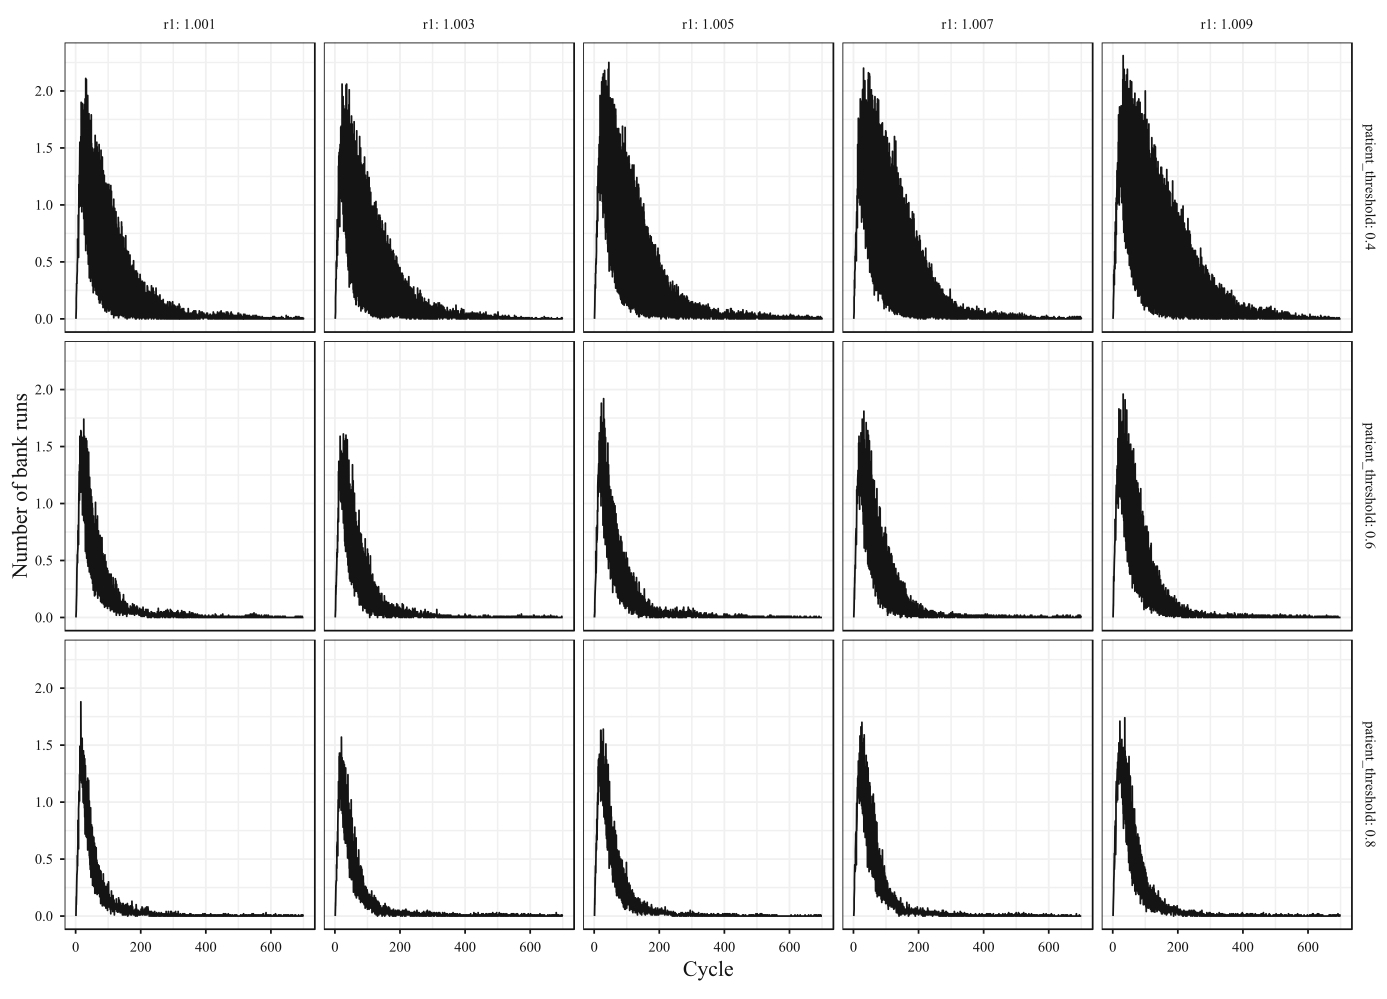
\includegraphics[width=\textwidth]{fig/fig3.jpeg}
        \caption{Average number of bank runs}
        \label{fig:num_run}
    \end{figure}
\end{frame}

\begin{frame}[plain]
    \begin{figure}
        \centering
        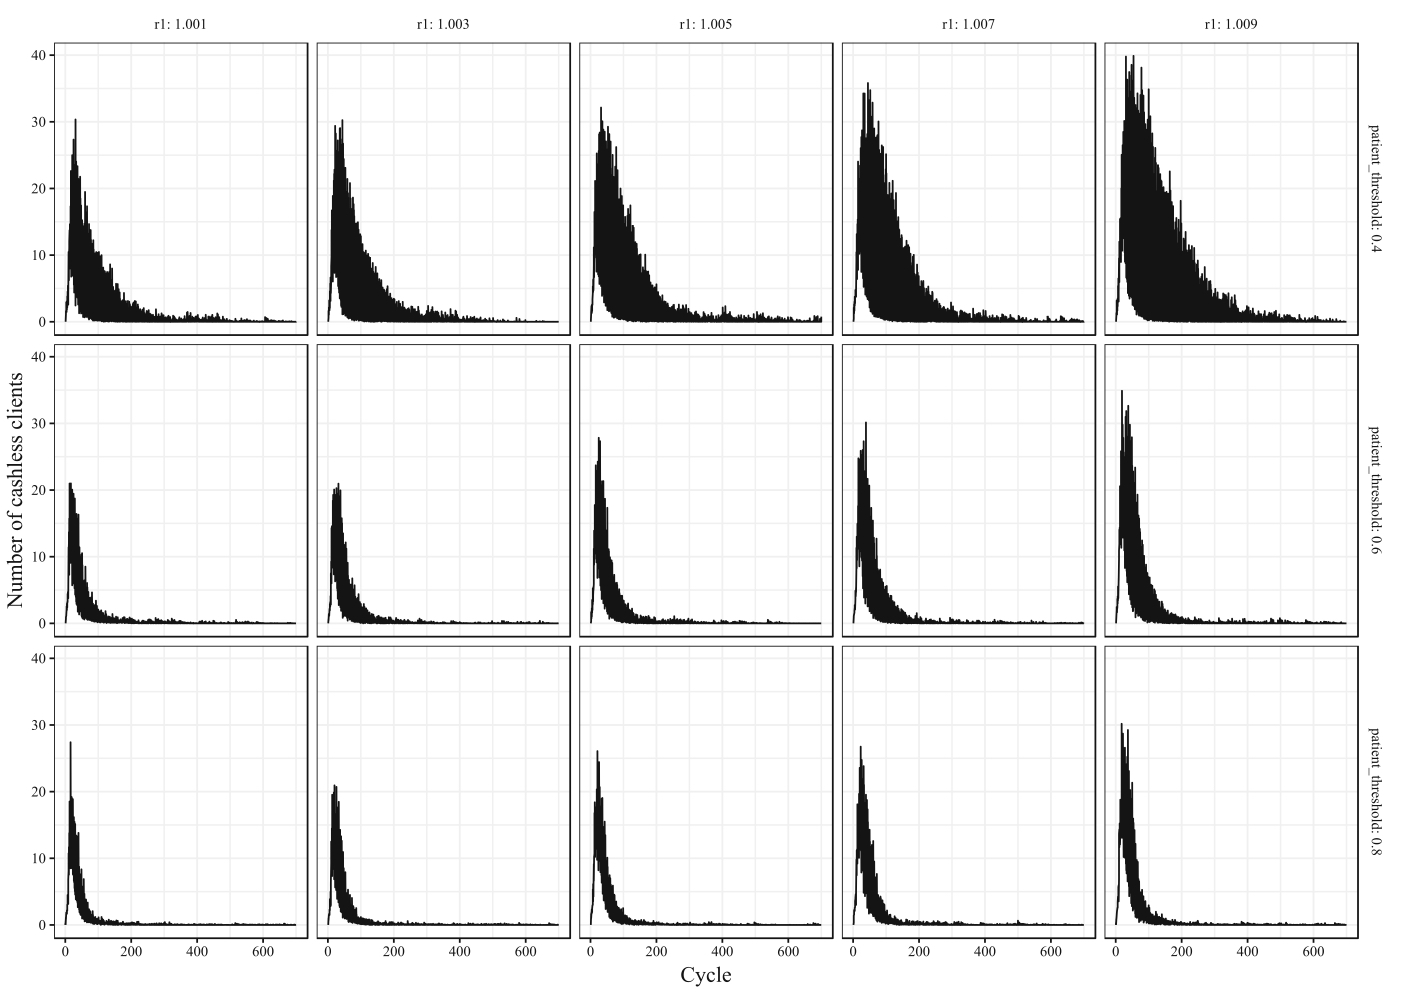
\includegraphics[width=\textwidth]{fig/fig4.jpeg}
        \caption{Average number of clients failed to withdraw}
        \label{fig:num_run}
    \end{figure}
\end{frame}

\begin{frame}[plain]
    \begin{figure}
        \centering
        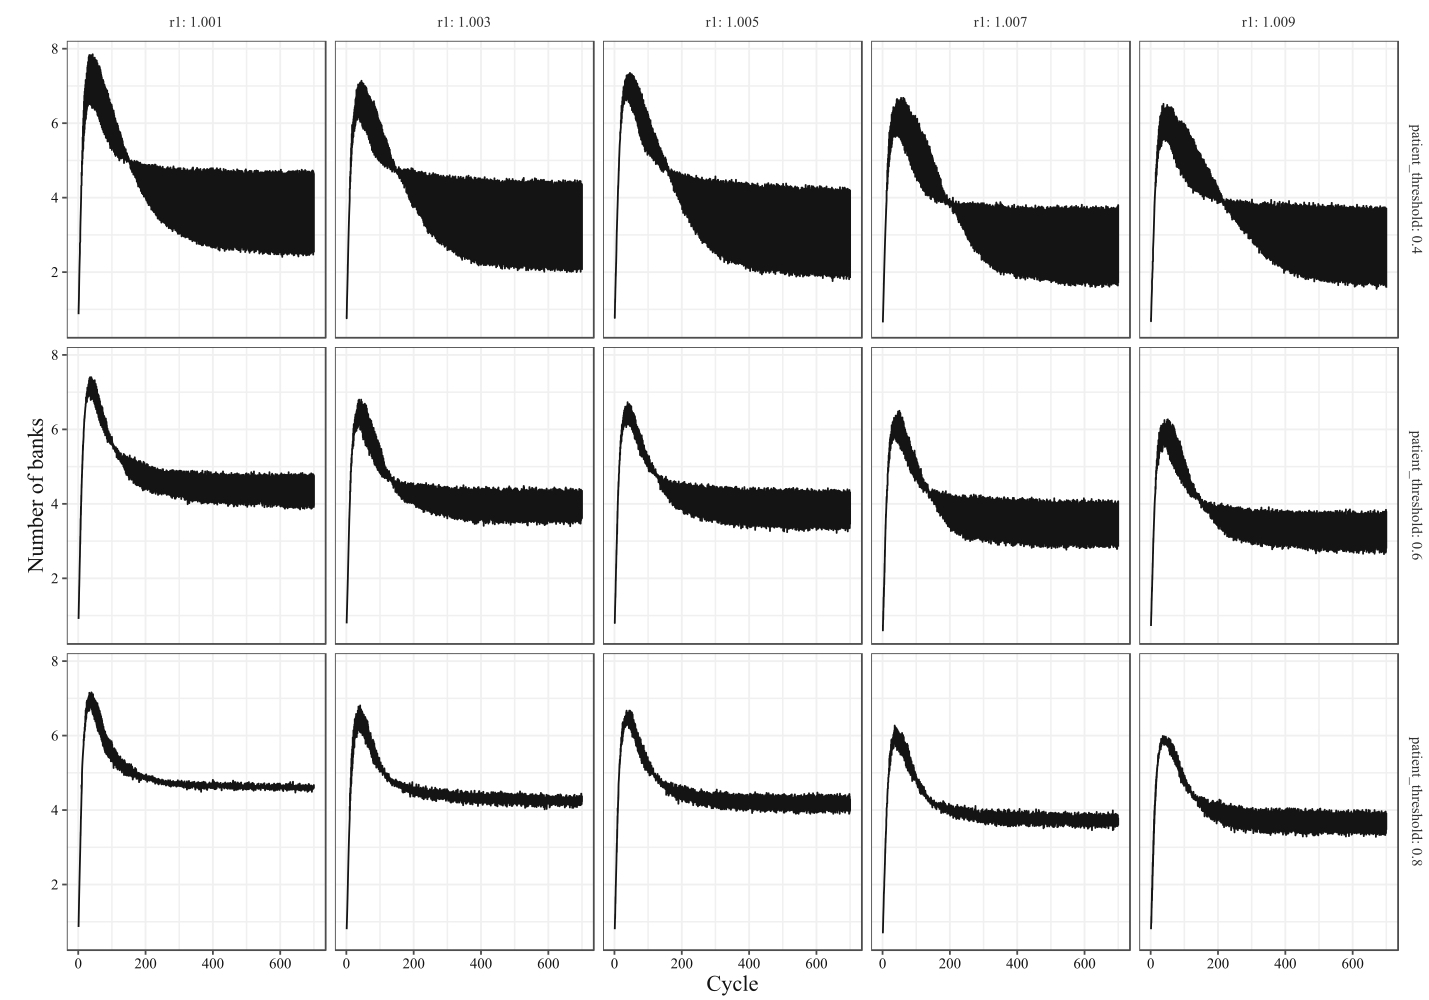
\includegraphics[width=\textwidth]{fig/fig5.jpeg}
        \caption{Average number of banks}
        \label{fig:num_run}
    \end{figure}
\end{frame}

\setcounter{figure}{6}

\begin{frame}[plain]
    \begin{figure}
        \centering
        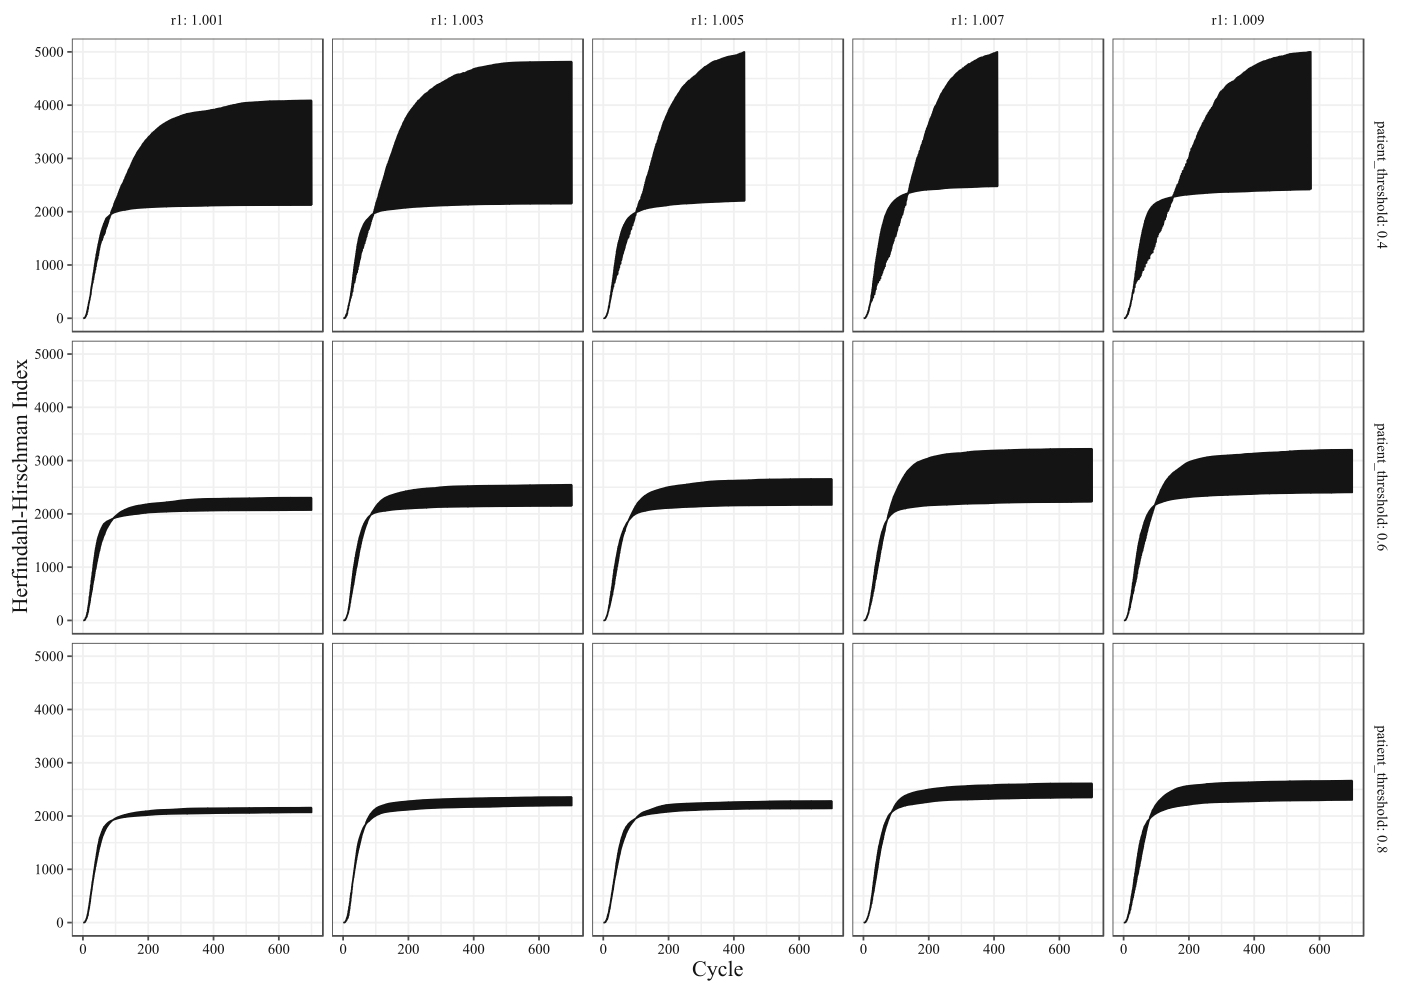
\includegraphics[width=\textwidth]{fig/fig7.jpeg}
        \caption{Average Herfindahl-Hirschman index (Sum of market share squared)}
        \label{fig:num_run}
    \end{figure}
\end{frame}


\begin{frame}[plain]
    \begin{figure}
        \centering
        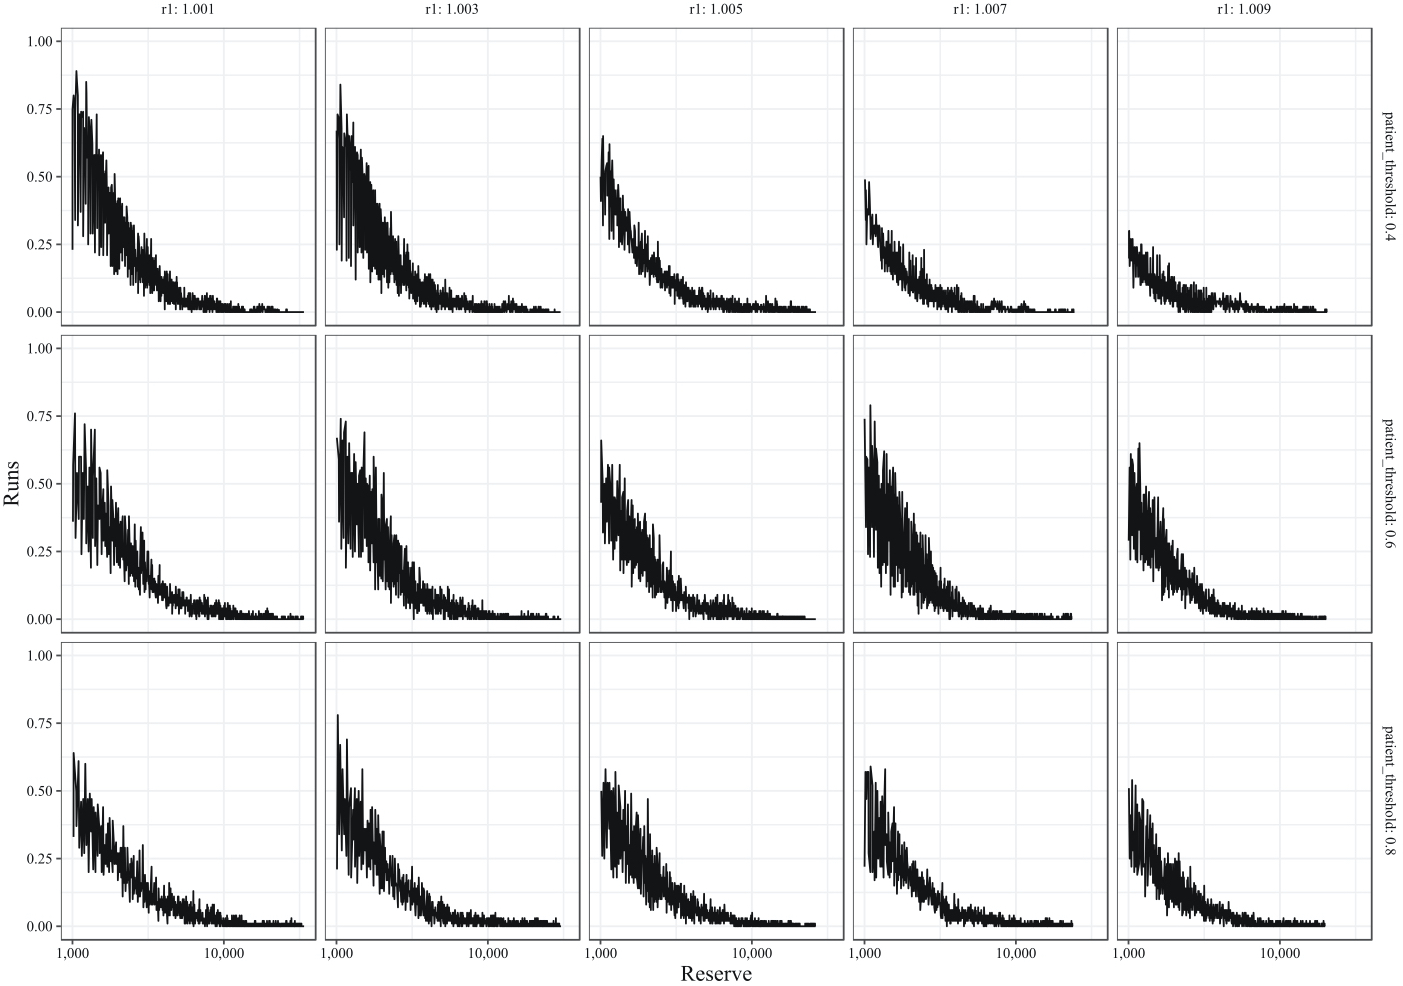
\includegraphics[width=\textwidth]{fig/fig8.jpeg}
        \caption{Bank reserve versus number of runs}
        \label{fig:num_run}
    \end{figure}
\end{frame}